% !TeX document-id = {0b75489a-6e79-4ace-8cb1-4028f93ab758}
% !TEX encoding = UTF-8 Unicode
% !TeX spellcheck = pl_PL
% !TEX TS-program = xelatex
% !TeX TXS-program:bibliography = txs:///biber
% !TeX TXS-program:index = txs:///makeindex

\documentclass[skorowidz,skroty]{dyplomWEZUT}
\usepackage{makecell}
\usepackage{float}
% ------------------------------------------------------------------------------
% Opcje klasy <dyplomWEZUT>
% 1) skorowidz - włącza skorowidz
% 2) skroty    - włącza wykaz ważniejszych skrótów i oznaczeń
% ------------------------------------------------------------------------------
\lstdefinelanguage{JavaScript}{
  keywords={break, case, catch, continue, debugger, default, delete, do, else, finally, for, function, if, in, instanceof, new, return, switch, this, throw, try, typeof, var, void, while, with, const, let, enum, Record},
  morecomment=[l]{//},
  morecomment=[s]{/*}{*/},
  morestring=[b]',
  morestring=[b]",
  sensitive=true
}

% -------------------------- Dane pracy dyplomowej -----------------------------

% Imię i Nazwisko
\author{Łukasz Aniszewski}

% Numer albumu
\nralbumu{36705}

% Tytuł pracy
\title{Aplikacja na smartphone prezentująca parametry rejsu jednostki pływającej}
% 
% Tytuł pracy w języku angielskim
\tytulang{SMARTPHONE APPLICATION THAT PRESENTS THE PARAMETERS OF THE VESSEL'S VOYAGE}

% Kierunek studiów
\kierunek{Automatyka i~Robotyka}

% Rodzaj studiów: S1/S2/N1/N2
\rodzajstudiow{S1}

% Data wydania tematu w SIWE/eDziekanacie
\datawydania{28.02.2020}

% Data dopuszczenia pracy do egzaminu (wypełnia Dziekanat)
\datazlozenia{......................................}

% Miejsce złożenia pracy (odkomentować i wypełnić jeżeli inne niż Szczecin)
%\miejsce{}

% Rok złożenia pracy (zmienić, jeśli inny niż 2020)
\date{2020}

% Imię i nazwisko opiekuna - wpisujemy w dopełniaczu
% Proszę zwrócić uwagę na kropkę po "dr" w dopełniaczu, jeśli opiekun jest mężczyzną
% Dopuszczalny jest również zapis "dra" bez kropki, w przypadku kobiety zawsze "dr" bez kropki 
\opiekun{dr inż. Robert Krupiński}

% Katedra, Instytut, Zakład lub Zespół Dydaktyczny
% (Wydział wpisujemy po przecinku tylko jeśli inny niż WE)
\jednostka{Katedra Przetwarzania Sygnałów i Inżynierii Multimedialnej}

% Słowa kluczowe
\slowakluczowe{NMEA, aplikacja mobilna, wizualizacja}

% Słowa kluczowe po angielsku
\keywords{NMEA, mobile application, visualization}

%% ----------------------- Koniec definicji danych -----------------------------

% Dodanie metadanych do wynikowego pdf (Autor, Tytuł, Słowa kluczowe)
\makemetadata

\begin{document}

\begin{streszczenie}
Celem pracy były stworzenie aplikacji prezentującej aktualne parametry jednostki pływającej. Zakres wykonanych prac obejmował przegląd aktualnie stosowanych rozwiązań, zapoznanie się i opis protokołu NMEA (National Marine Electronics Association) oraz część oprogramowania aplikacji mobilnej. Dla testów skorzystano z dostępnego w sieci symulatora jednostki wysyłającej dane zakodowane protokołem NMEA. Głównymi z napotkanych problemów były – ilość oraz dokumentacja komend protokołu NMEA, przygotowanie oprogramowania pod łatwy rozwój o wsparcie dla kolejnych komend. Podczas wyboru technologii kierowano się głównie osobistym doświadczeniem oraz umiejętnościami. 
\end{streszczenie}

\begin{abstract}
The aim of the work was to create a mobile application for presenting actual parameters ofthe vessel's voyage. The scope of work included an overview of actually used solutions, acquiring the knowledge about NMEA (National Marine Electronics Association) protocol and describing it, creating software for mobile application. For testing purposes, NMEA Simulator (available on the internet) which sends NMEA encoded data was used. The main encountered issues were – the amount and documentation of NMEA protocol sentences, preparing the software for easy expansion by additional sentences. The choice of the technological stack was mainly based on personal experience and skills.
\end{abstract}

\maketitle

\begin{wprowadzenie}

Komunikacja między urządzeniami elektronicznymi jest obecnie standardem. Zależnie od obszaru działań wspomnianych urządzeń stosowane są odmienne protokoły. Jednostki pływające, których dotyczy ta praca korzystają ze standardu \textit{NMEA}. Brak jednak narzędzi pozwalających w łatwy sposób przedstawić człowiekowi dane zakodowane tym protokołem. Obecnie aplikacje mobilne stanowią ogromną część rynku oprogramowania. Niemal każdy posiada smartphone i korzysta z aplikacji dla systemów takich jak \textit{Android} czy \textit{iOS}. W kolejnych rozdziałach został przedstawiony proces tworzenia takiej aplikacji. Równie dużą, a nawet większą, rolę odgrywa obecnie komunikacja sieciowa, większość znanych nam stron i aplikacji bazuje na architekturze \textit{REST}, popularność zyskuje \textit{GraphQL}, a do określonych zadań stosuje się protokoły takie jak \textit{WebSocket}. Właśnie ten ostatni został wykorzystany w pracy, co zostanie przedstawione w kolejnych rozdziałach. 

\end{wprowadzenie}

\cel{Celem pracy jest stworzenie aplikacji mobilnej prezentującej aktualne parametry jednostki pływającej.}

\zakres{Zakres pracy obejmuje Przegląd aktualnie stosowanych rozwiązań w zakresie parametrów jednostek pływających oraz metod ich prezentacji, zapoznanie się i opisanie standardu dla protokołu \textit{NMEA} (National Marine Electronics Association) oraz stworzenie aplikacji mobilnej na Smartphone wraz z \textit{GUI} (Graphical User Interface) prezentującej aktualne parametry jednostki pływającej z wykorzystaniem sieci \textit{WiFi} jednostki pływającej. Celem dodatkowym jest przetestowanie aplikacji w warunkach rzeczywistych na jednostce pływającej.} 

\chapter{Protokół NMEA}\label{chap:NMEA protocol}

Komunikacja między morskimi urządzeniami elektronicznymi wykorzystuje protokół \textit{NMEA}. Wyróżniamy dwie wersje tego protokołu – \textit{NMEA 0183} oraz \textit{NMEA 2000} \cite{NMEA0183Standard, NMEA2000Standard}. Obecnie interfejs \textit{NMEA 0183} zastępowany jest przez nowszy \textit{NMEA 2000}, jednak praca dotyczy będącego przez lata standardem oraz ciągle wykorzystywanego starszego protokołu. Odniesienia do protokołu \textit{NMEA} w dalszej części pracy oznaczać będą wersję 0183. 

\section{Format komendy NMEA}\label{sec:format nmea}

Na podstawie \cite{NMEA0183} należy wydzielić podstawowe typy komend: talker sentences (źródeł danych), proprietary sentences (zdefiniowanych przez poszczególnych producentów), query sentences (zapytań). Pierwszy typ, na którym skupia się ta praca, obejmuje sygnały GPS,  dane z urządzeń wbudowanych w jednostkę, czujników. Typ drugi pozwala indywidualnym producentom zdefiniować własne formaty, linie danych tego typu zaczynają się od znaków \texttt{„\$P”} poprzedzających trzy literowy identyfikator producenta. Następnie zawarte są dane, o których decyduje producent. Ostatni typ pozwala urządzeniu zażądać wybranego rodzaju komendy od innego urządzenia. Ogólne formaty wyglądają następująco:
\begin{enumerate}
\item Talker Sentence - \texttt{\$ttsss,d1,d2,....<CR><LF>}, gdzie „tt” oznacza identyfikator nadawcy, „sss” identyfikator komendy, a „d1, d2…” kolejne pola danych. 
\item Proprietary Sentence - \texttt{\$Psss,d1,d,2,…<CR><LF>}, gdzie „sss” oznacza identyfikator producenta, a „d1,d2...” kolejne pola danych.
\item Query Sentence - \texttt{\$ttllQ,sss,<CR><LF>}, gdzie „tt” oznacza identyfikator żądającego, „ll” identyfikator urządzenia, do którego zostało skierowane zapytanie, a „sss” identyfikator żądanej komendy.
\end{enumerate}
Każda linia danych nadana w protokole \textit{NMEA} zaczyna się od znaku „\$”, dane oddzielone są przecinkami, a komenda kończy się sumą kontrolną poprzedzoną znakiem „*”.

\section{Identyfikatory nadawców}\label{sec:talker ids}
Identyfikatory nadawców rozróżniają linie danych \textit{NMEA} ze względu na źródło informacji, o których mowa w danej komendzie.

\code{Identyfikatory nadawców}
{Opracowanie własne \cite{gpsinformation, Raymond2019}}{\label{code:Talkers enum}}
\begin{lstlisting}[language=JavaScript]
enum TalkerIdentifiers {
    AG= 'AG', AP= 'AP', CD= 'CD', CR= 'CR', CS= 'CS', CT= 'CT', CV= 'CV',
    CX= 'CX', DF= 'DF', EC= 'EC', EP= 'EP', ER= 'ER', GP= 'GP', HC= 'HC',
    HE= 'HE', HN= 'HN', II= 'II', IN= 'IN', LC= 'LC', RA= 'RA', SD= 'SD',
    SN= 'SN', SS= 'SS', TI= 'TI', VD= 'VD', DM= 'DM', VW= 'VW', WI= 'WI',
    YX= 'YX', ZA= 'ZA', ZC= 'ZC', ZQ= 'ZQ', ZV= 'ZV'
}
\end{lstlisting}

\code{Deskryptory nadawców}
{Opracowanie własne na podstawie \cite{gpsinformation, Raymond2019}}{\label{code: talkers descriptors}}
\begin{lstlisting}[language=JavaScript]
const TalkerDescriptors: Record<TalkerIdentifiers, string> = {
    [TalkerIdentifiers.AG]: 'Autopilot - General',
    [TalkerIdentifiers.AP]: 'Autopilot - Magnetic',
    [TalkerIdentifiers.CD]: 'Communications - Digital Selective Calling (DSC)',
    // deskryptor uległa skróceniu w celach edytorskich
    [TalkerIdentifiers.ZC]: 'Timekeeper - Chronometer',
    [TalkerIdentifiers.ZQ]: 'Timekeeper - Quartz',
    [TalkerIdentifiers.ZV]: 'Radio Update, WWV or WWVH'
};
\end{lstlisting}

\section{Identyfikatory komend}\label{sec:sentence ids}
Lista wspieranych przez aplikację identyfikatorów komend.
\code{Identyfikatory komend}
{Opracowanie własne na podstawie \cite{gpsinformation, Raymond2019}}{\label{code:Sentences enum}}
\begin{lstlisting}[language=JavaScript]
enum SentenceIdentifiers {
    AAM= 'AAM', ALM= 'ALM', APA= 'APA', APB= 'APB', ASD= 'ASD', BEC= 'BEC',
    BOD= 'BOD', BWC= 'BWC', BWR= 'BWR', BWW= 'BWW', DBK= 'DBK', DBS= 'DBS',
    DBT= 'DBT', DCN= 'DCN', DPT= 'DPT', DSC= 'DSC', DSE= 'DSE', DSI= 'DSI',
    DSR= 'DSR', DTM= 'DTM', FSI= 'FSI', GBS= 'GBS', GGA= 'GGA', GLC= 'GLC',
    GLL= 'GLL', GRS= 'GRS', GST= 'GST', GSA= 'GSA', GSV= 'GSV', GTD= 'GTD',
    GXA= 'GXA', HDG= 'HDG', HDM= 'HDM', HDT= 'HDT', HSC= 'HSC', LCD= 'LCD',
    MSK= 'MSK', MSS= 'MSS', MWD= 'MWD', MTW= 'MTW', MWV= 'MWV', OLN= 'OLN',
    OSD= 'OSD', ROO= 'ROO', RMA= 'RMA', RMB= 'RMB', RMC= 'RMC', ROT= 'ROT',
    RPM= 'RPM', RSA= 'RSA', RSD= 'RSD', RTE= 'RTE', SFI= 'SFI', STN= 'STN',
    TLL= 'TLL', TRF= 'TRF', TTM= 'TTM', VBW= 'VBW', VDR= 'VDR', VHW= 'VHW',
    VLW= 'VLW', VPW= 'VPW', VTG= 'VTG', VWR= 'VWR', WCV= 'WCV', WDC= 'WDC',
    WDR= 'WDR', WNC= 'WNC', WPL= 'WPL', XDR= 'XDR', XTE= 'XTE', XTR= 'XTR',
    ZDA= 'ZDA', ZDL= 'ZDL', ZFO= 'ZFO', ZTG= 'ZTG'
}
\end{lstlisting}

\code{Deskryptory komend}
{Opracowanie własne na podstawie \cite{gpsinformation, Raymond2019}}{\label{code: sentences descriptors}}
\begin{lstlisting}[language=JavaScript]
const SentencesDescriptions: Record<SentenceIdentifiers, string> = {
    [SentenceIdentifiers.AAM]: 'Waypoint Arrival Alarm',
    [SentenceIdentifiers.ALM]: 'GPS Almanac Data',
    [SentenceIdentifiers.APB]: 'Autopilot Sentence "B"',
    // deskryptor uległa skróceniu w celach edytorskich
    [SentenceIdentifiers.ZDL]: 'Time & Distance to Variable Point',
    [SentenceIdentifiers.ZFO]: 'UTC & Time from Origin Waypoint',
    [SentenceIdentifiers.ZTG]: 'UTC & Time to Destination Waypoint'
};
\end{lstlisting}

\section{Komendy ujęte w aplikacji}\label{sec:application sentences}
Z racji bardzo dużej ilości istniejących komend protokołu \textit{NMEA} do realizacji pracy inżynierskiej zostały wybrane linie danych uwzględnione w używanym symulatorze \textit{NMEA Simulator}. Oznacza to pełne dekodowanie oraz wyświetlanie danych w nich zawartych, jednak aplikacja została stworzona w taki sposób, aby dodawanie kolejnych komend było jak najprostsze. Szczegóły zostaną omówione w dalszym rozdziale. Dane dostarczone przez symulator opisują zarówno położenie jak i dane na temat samej jednostki. Na ich podstawie zbudowany został interfejs graficzny aplikacji. Pełna lista znajduje się w tabeli 1.1.

\tabela{Komendy \textit{NMEA} w pełni dekodowane przez aplikacje\label{tab:application sentences table}}
{Opracowanie własne}
{\begin{tabular}{c|c|c|c}
\thead{Identyfikator \\ nadawcy} & Nadawca & \thead{Identyfikator \\ komendy} & Komenda \\\hline\hline
SD & Sounder & DBT & Depth below transducer\\
\hline
GP & \makecell{Global Positioning \\ System (GPS)} & GGA & Global Positioning System Fix Data\\
\hline
GP & \makecell{Global Positioning \\ System (GPS)} & GSA & GPS DOP and active satellites\\
\hline
II & Integrated instrumentation & MTW & Mean Temperature of Water\\
\hline
WI & Weather Instruments & MWD & Wind Direction and Speed\\
\hline
WI & Weather Instruments & MWV &  Wind Speed and Angle\\
\hline
GP &\makecell{Global Positioning \\ System (GPS)} & RMC & \makecell{Recommended Minimum \\ Navigation Information}\\
\hline
II & Integrated instrumentation & VHW & Water speed and heading
\end{tabular}}

\chapter{Przegląd dostępnych rozwiązań}\label{chap: Available solutions}

Gałąż przemysłu (biznesu) morskiego może być uważana za sektor, gdzie bezpieczeństwo gra odgórną rolę, stąd standard \textit{NMEA} definiuje także warstwę elektryczną interfejsu i w tym przypadku jest to \textit{EIA-422} - czyli połączenie z jednym masterem oraz wieloma slave'ami. Istnieje także standard, który mówi o pakowaniu ramek \textit{NMEA} w datagram UDP - ale nie opisuje go formalnie żaden dokument.

Chcąc dokonać kategoryzacji istniejących rozwiązań należałoby zastanowić się nad ograniczeniem ich spektrum, ponieważ wiele firm oferuje rozwiązania programowo-sprzętowe, które są gateway'em między fizycznym połączeniem \textit{EIA-422} (zdefiniowanym przez standard) - a siecią \textit{WiFi}. Przykładem takiego rozwiązania jest produkt \textit{WLN10 Smart} firmy \textit{DIGITAL YACHT} \cite{DIGITALYACHT} pozwalający na udostępnianie danych \textit{NMEA} przez \textit{WiFi}. Koszt tego produktu to 150£. W dalszej części omówione zostaną aplikacje wizualizujące owe dane .

\section{Rozwiązania darmowe}\label{chap: Free solutions}

Darmowe rozwiązania dostępne dla urządzeń mobilnych są w większości przypadków mocno ograniczone, niewspierane przez twórcę lub twórców, obarczone licznymi błędami. Przykładowe aplikacje:
\begin{enumerate}

\item \textit{NMEA Tools} \cite{NMEATools} ~Rysunek~\ref{fig:NMEA-Tools} w wersji darmowej pozwala na odczyt danych \textit{NMEA} z pliku tekstowego, co mocno ograniczna użyteczeność tego rozwiązania. 

\item \textit{NavMonitor} \cite{NavMonitor} ~Rysunek~\ref{fig:NavMonitor} wizualizuje dane dotyczące między innymi wiatru, pozycji, prędkości jednostki, czy temperatury oraz głębokości wody. Nie posiada jednak przedstawienia obiektu na mapie, co jest znaczącą wadą. 

\item \textit{SeaWi Marine} \cite{SeaWiMarine} ~Rysunek~\ref{fig:SeaWi-Marine} jest jednym z najbardziej rozbudowanych rozwiązań. Aplikacja oferuje wiele funkcjonalności, w tym wizualzację danych w formie zarówno graficznej, czyli przedstawione na mapie, jak i tekstowej w postaci zdekodowanych informacji. Pozwala na tworzenie punktów kontrolnych, konfigurację alarmów, a w tym także możliwość wysłania wiadomości SMS w przypadku ich wystąpienia, oraz wiele innych. Wadą jest niekompletny zestaw map, na chwilę obecną obejmujący Europę, Amerykę Północną, Morze Śródziemne, Morze Czarne, Karaiby, Australię, Nową Zelandię, Pacyfik oraz Afrykę Północną. Twórcy zapewniają, że mapy dla reszty świata zostaną dostarczone w przyszłości.

\rysunek{NMEA-Tools}
{NMEA Tools \label{fig:NMEA-Tools}}
{https://play.google.com/store/apps/details?id=com.peterhohsy.nmeatools}

\rysunek{NavMonitor}
{NavMonitor \label{fig:NavMonitor}}
{https://play.google.com/store/apps/details?id=com.aboni.boatinga}

\rysunek{SeaWi-Marine}
{SeaWi Marine \label{fig:SeaWi-Marine}}
{https://play.google.com/store/apps/details?id=net.seawimarine.activities}

\end{enumerate}
\newpage
\section{Rozwiązania komercyjne}\label{chap: Commercial solutions}

Płatne rozwiązania zrealizowane są w modelu jednorazowej płatności za oprogramowania lub konieczności wykupienia czasowej subskrypcji, aby uzyskać dostęp do pełni funkcjonalności. Najczęściej subskrypcją objęty jest dostęp do map. Przykładowe aplikacje:
\begin{enumerate}

\item \textit{iRegatta Pro} \cite{iRegatta} ~Rysunek~\ref{fig:iRegatta} pozwala na odczyt danych dotyczących między innymi wiatru, prędkości jednostki i jej położenia. Oprócz komunikacji sieciowej wspiera także komunikację przy wykorzystaniu \textit{BlueTooth}. Brakuje wizualizacji obiektu na mapie. Cena tej aplikacji wynosi 69,99 złotych.

\item \textit{Seapilot} \cite{Seapilot} ~Rysunek~\ref{fig:Seapilot} oferuje przede wszystkim pełen detali widok mapy, przeznaczony do specjalistycznego użycia. Podstawowe informacje na temat jednostki widoczne są w formie tekstowej. Dostęp do pełni funkcjonalności wymaga wykupienia licencji na stronie producenta. Cena wynosi 39,99\$ rocznie. Dodatkowo należy wykupić mapy obejmujące interesujące użytkownika rejony, również opłacane rocznie.

\item \textit{NMEAremote} \cite{NMEAremote} ~Rysunek~\ref{fig:NMEAremote} podobnie jak konkurencja przedstawienie zdekodowanych danych w przyjaznej dla użytkownika formie. Brakuje przedstawienia obiektu na mapie. Twórcy zapewniają listę wspieranych komend protokołu \textit{NMEA 0183} oraz \textit{NMEA 2000}. Jest to odpowiednio trzydzieści siedem oraz dziewiętnaście typów komend. Kosz aplikacji wynosi 17,99\$.  

\end{enumerate}

\begin{figure}[H]
  \centering
    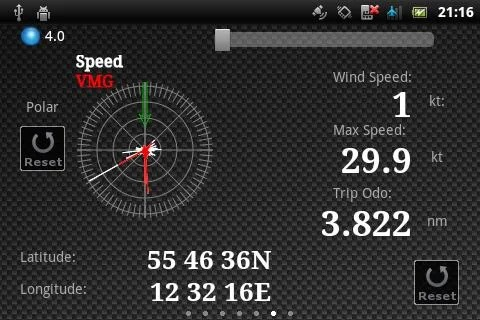
\includegraphics[scale=1.0]{graphic/iRegatta}
    \caption{\textit{iRegatta}}
    \source{https://play.google.com/store/apps/details?id=dk.letscreate.aRegatta}
    \label{fig:iRegatta}
\end{figure}

\begin{figure}[H]
  \centering
    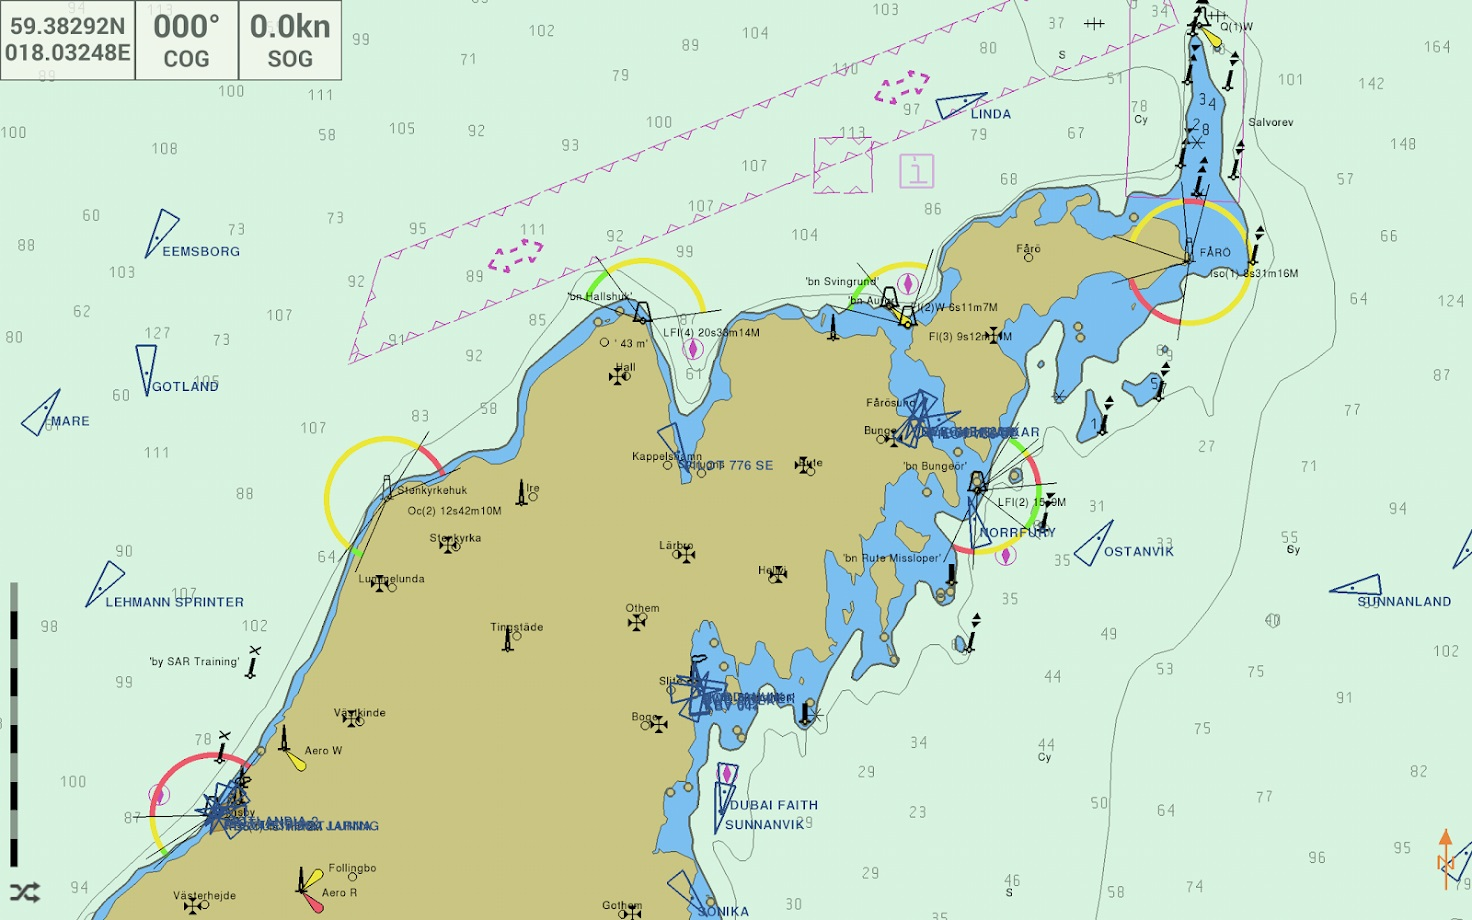
\includegraphics[scale=0.3]{graphic/Seapilot}
    \caption{\textit{Seapilot}}
    \source{https://play.google.com/store/apps/details?id=com.seapilot.android}
    \label{fig:Seapilot}
\end{figure}

\begin{figure}[H]
  \centering
    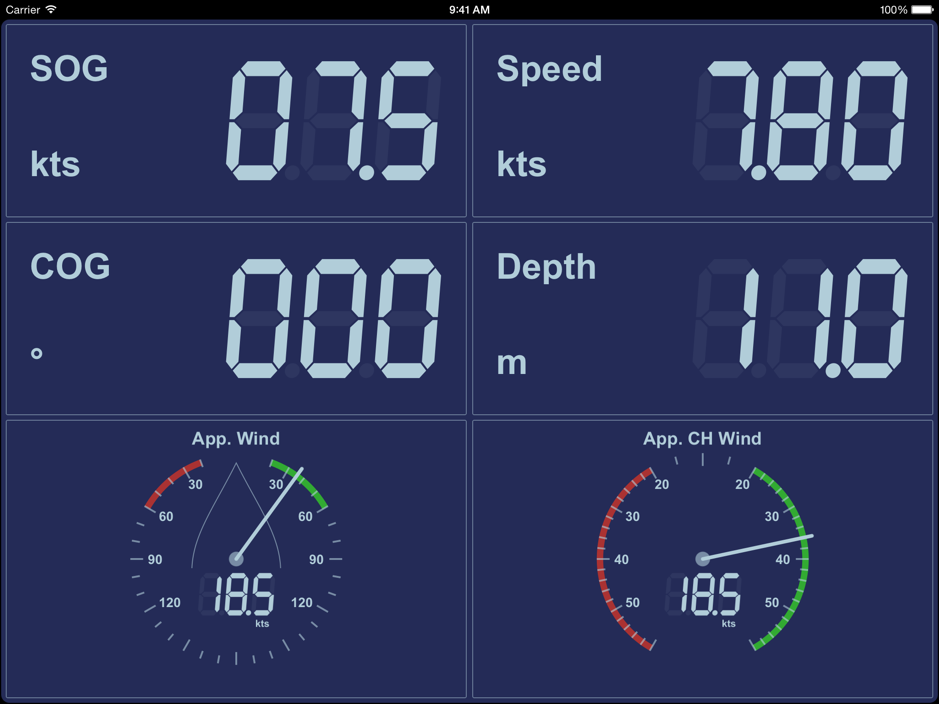
\includegraphics[scale=0.3]{graphic/NMEAremote}
    \caption{\textit{NMEAremote}}
    \source{https://apps.apple.com/us/app/nmearemote/id412806204}
    \label{fig:NMEAremote}
\end{figure}

\section{Podsumowanie}\label{chap: summary}

Dostępne rozwiązania nie są perfekcyjne, jednak w przybliżeniu pokrywają się z celem pracy. Wiele dostępnych aplikacji zostało pomięte w tym rozdziale z uwagi na olbrzymią liczbę negatywnych komentarzy użytkowników, często implikujących całkowitą niezdatność oprogramowania do użytku. Aby uzyskać w pełni spersonalizowane rozwiązanie należy je stworzyć. W kolejnym rozdziale przedstawiony został sposób doboru narzędzi oraz motywy stojące za poszczególnymi wyborami, a także proces tworzenia aplikacji wraz z wyszczególnieniem głównych konceptów kodu źródłowego.

\chapter{Aplikacja Mobilna}\label{chap:Mobile App}

\section{Język programowania}\label{sec: language}
Domena tworzenia oprogramowania jest bardzo obszerna i może być dzielona wedle różnych kryteriów. Pierwszą przychodzącą na myśl kategoryzacją jest podział ze względu na różne języki programowania, te najbardziej popularne z nich, czyli \textit{C}, \textit{C++}, \textit{Python}, \textit{Java}, \textit{C\#}, \textit{JavaScript} są wystarczająco odmienne, aby było to adekwatne kryterium. Innym, prawdopodobnie najbardziej szczegółowym zbiorem kryteriów są kryteria techniczne. Najważniejsze z nich to:
\begin{enumerate}

\item Sposób egzekucji (czyli sposób, w jaki wykonywany jest dany program komputerowy):
\begin{itemize}
	\item Języki interpretowalne, czyli takie, w których środowiskiem działania jest wirtualna maszyna a kod w sposób dynamiczny wykonywany jest linijka po linijce bez translacji na kod maszynowy danego procesora
	\item Języki kompilowalne, czyli takie, w których do uruchomienia programu wymagana jest zamiana jego postaci na kod wykonywalny, zrozumiały dla danej architektury
	\item Języki hybrydowe, czyli będącę połączeniem powyższych dwóch - przykładowo, niektóre fragmenty kodu są kompilowane (najczęściej tam gdzie zależy nam na optymalności rozwiązania)
\end{itemize}

\item Wspierany paradygmat programowania, głównie:
\begin{itemize}
	\item Structural Programming (SP), czyli paradygmat, który za podstawowy element budulcowy uznaje funkcje (procedury), które są zbiorem instrukcji, które mają wpływ na stan programu. Całość jest hierarchiczna oraz sekwencyjna. Pierwszym najszerzej rozpowszechnionym, uznanym i do dzisiaj używanym językiem strukturalnym jest język \textit{C}
	\item Object Oriented Programming (OOP), czyli próba opisania oprogramowania w sposób jak najbardziej oddający otaczający nas świat. Klasy oraz obiekty stanowią warstwę abstrakcji reprezentującą dane procesy oraz podmioty. Wedle definicji możemy wymienić cztery filary programowania obiektowego: abstrakcja, hermetyzacja, polimorfizm oraz dziedziczenie. Obecnie jest to dominujący na rynku paradygmat, cechujący przede wszystkim \textit{C++}, \textit{C\#} i \textit{Java}. Nie jest jednak pozbawiony wad oraz problemów wynikających z samych jego założeń. 
	\item Functional Programming (FP), czyli paradygmat można rzec inspirowany matematyką. W jego podstawowych założeniach kod źródłowy składałby się z wielu przewidywalnych funkcji, nazywanych 'pure functions'. Takie funkcje muszą zawsze zwracać dokładnie taki sam rezultat przy takich samych danych wejściowych, niezależnie od jakichkolwiek innych czynników. Tak restrykcyjne założenie uniemożliwia wywoływanie jakichkolwiek efektów ubocznych (ang. side effects) w kodzie, czego najbardziej dobitnym przykładem są operacje I/O będące podstawą znakomitej części oprogramowań. Chciałbym tutaj zaznaczyć, że wbrew rozumowaniu wielu inżynierów oprogramowania, nie oznacza niemożliwości wykorzystania efektów ubocznych. W językach programowania funkcyjnego jest to w pełni możliwe, a sam paradygmat dopuszcza łamanie założeń w niezbędnych operacjach. Programowanie funkcyjne posiada wysoki próg wejścia, może wydawać się nieintuicyjne i skomplikowane oraz przestarzałe. Zyskuje jednak ponownie na popularności, powoli stając się konkurentem dla programowania obiektowego. Przykładowe języki reprezentujące ten paradygmat to \textit{Haskell}, \textit{Lisp}.
\end{itemize}  

\item Typowanie:
\begin{itemize}
	\item Statyczne, inaczej zwane twardo typowanym, języki tego typu wymagają od programisty znajomości i deklaracji typów danych. Cechujące wszystkie najstarsze języki programowania, a także większość obecnie używanych. Zapewnia możliwość znalezienia błędów ludzkich na poziomie kompilacji, czyli bez konieczności uruchamiania i sprawdzania oprogramowania. Przykładowe języki: \textit{C}, \textit{C++}, \textit{Java}, \textit{C\#}
	 \item Dynamiczne, inaczej zwane miękko typowanym, języki tego typu nie posiadają oznaczeń typów danych, takich jak np. 'string' czy 'float', lub nie wymagają jawnego ich podawania. Zaletą takiej konwencji jest mniejsza ilość kodu oraz większa przystępność dla początkujących programistów. Przykładowe języki: \textit{Python}, \textit{JavaScript}. 

\end{itemize}

\end{enumerate} 
Kolejnym logicznym kryterium jest docelowa platforma, dzięki czemu wyróżnimy programowanie wbudowane, web'owe, desktop'owe, mobilne. Należy zauważyć, że w tym wypadku niektóre z wyżej wymienionych języków trafią do wspólnego zbioru. Dla przykładu zarówno \textit{Python} jak i \textit{JavaScript} można nazwać językami web'owymi (lecz nie tylko). Pojawia się tutaj pewien problem, którym jest skalowanie oprogramowania. Jeśli firma posiada obiecujące oprogramowanie to ograniczenie grona odbiorców do danej platformy jest bardzo niekorzystne. Z między innymi tego powodu, języki programowania ewoluowały stając się wieloplatformowe. Dla przykładu \textit{Java}, będąca jednym z najpopularniejszych języków na rynku, została stworzona z założeniem wsparcia różnych platform bez potrzeby ingerowania w kod. 

Wyżej wymienione kryteria mają olbrzymie znaczenie podczas wyboru języka dla danego projektu. W przypadku aplikacji będącej podmiotem pracy inżynierskiej zdecydowano się na \textit{TypeScript}, czyli nadzbiór języka \textit{JavaScript}. Podobnie jak \textit{JavaScript} wspiera on zarówno programowanie funkcyjne jak i obiektowe. Natomiast najistotniejszymi różnicami są kompilacja oraz wsparcie dla twardego typowania. Kompilowany jest on do czystego \textit{JavaScript}, który następnie interpretowany jest przez środowisko klienckie, czyli np. \textit{node.js} lub przeglądarka internetowa. Dzięki temu w przypadku, gdy nie jesteśmy w stanie lub nie chcemy określać typu danych - jest to całkowicie dozwolone. Przykładowo - dane dostarczane z zewnętrznej biblioteki, której twórca nie zapewnia ich struktury. W przypadku niektórych frameworków wymuszone jest użycie języka \textit{TypeScript}, w innych jest to opcjonalne. Przykładowo jeden z najpopularniejszych frameworków do tworzenia \textit{GUI} o nazwie \textit{Angular} wymusza używanie tej technologii. Podobnie jak zyskujący coraz większą popularność \textit{NestJS}, służący do tworzenia aplikacji serwerowych. Po wybraniu języka programowania przychodzi czas na wybór frameworka, który usprawni pracę.

\section{Framework}\label{sec: framework}

Framework dostarcza programiście szkielet aplikacji, a także metody, komponenty, serwisy oraz składnię do ich wykorzystywania. Wedle statystyki przedstawionej na ~Rysunek~\ref{fig:Frameworks_statictics} \cite{FrameworksPopularity} najpopularniejszym z frameworków do tworzenia aplikacji webowych po stronie klienta jest \textit{ReactJs}, konkurujący z frameworkami nazwanymi \textit{Angular} oraz \textit{Vue}. Nie udostępnia on jednak możliwości tworzenia natywnych aplikacji mobilnych na systemy \textit{Android} oraz \textit{iOS}. Na te potrzeby powstał \textit{ReactNative}. Jest to odpowiednik wspomnianego \textit{ReactJs} dedykowany dla platform mobilnych. Podstawowe założenia takie jak kompozycja komponentów, przesyłanie danych, czy cykl życia komponentu pozostają bez zmian. Znaczące różnice wynikają z faktu, że w odróżnieniu do przeglądarek, aplikacje mobilne nie wspierają składni \textit{HTML} oraz \textit{CSS}. Na podstawie \cite{ReactNative} w miejsce pierwszego \textit{ReactNative} dostarcza podstawowe komponenty pozwalające na budowanie widoku. Odpowiednikiem elementu \textit{<div />} w składni \textit{HTML} jest w tym wypadku element \textit{<View />}. Olbrzymią zaletą tego frameworka jest fakt, że w podanym przykładzie element \textit{<View />} zostanie wyrenderowany przy użyciu natywnego \textit{API} platformy, co zapewnia dużo lepszą wydajność w porównaniu do przykładowo frameworku\textit{Cordova}, który do renderowania wykorzystuje \textit{WebView}. ~Rysunek~\ref{fig:react-native} Arkuszy Styli \textit{CSS} zastąpione są natomiast przez obiekty \textit{Stylesheets}. Zaletą takiego podejścia jest możliwość przeniesienia aplikacji napisanej w \textit{ReactNative} na \textit{ReactJS} przy stosunkowo niewielkim nakładzie pracy, gdyż znaczna część kodu może zostać użyta ponownie. 
Dodatkowo został wykorzystany framework oraz platforma \textit{Expo}. Wedle \cite{Expo} jest to zbiór narzędzi oraz serwisów zbudowanych wokół \textit{ReactNative}, mający na celu przyspieszenie procesu tworzenia aplikacji. Dostarcza on między innymi przydatne warstwy abstrakcji nałożone na natywne \textit{API}, przykładowo dostęp do kamery, czy żyroskopu. Dodatkowo zapewnia rozbudowane \textit{CLI} (Command Line Interface). Jedną z jego możliwości jest niezwykle proste budowanie kodu na określoną platformę oraz serwer deweloperski z funkcją 'hot-reload'. Oznacza to, że zapisanie zmiany w kodzie natychmiast wywoła proces budowy odpowiednich plików, a programista ma możliwość obserwowania zmian na bieżąco używając symulatora urządzenia mobilnego lub rzeczywistego urządzenia. Sam proces połączenia z serwerem deweloperskim jest niesłychanie prosty. \textit{Expo} dostarcza adres url zawierający pliki źródłowe. Dla ułatwienia jest on również przedstawiony jak kod QR. Dowolne urządzenie mobilne posiadające aplikację kliencką \textit{Expo} po zeskanowaniu tego kodu uruchomi wersję deweloperską aplikacji. ~Rysunek~\ref{fig:expo} Oczywiście takie udogodnienia nakładają pewne ograniczenia, przez co dla dużych projektów z rozbudowaną logiką biznesową Expo może okazać się niewłaściwym wyborem. Jednak analiza pod kątem potrzeb omawianej pracy pozwoliła na uzasadniony wybór tego narzędzia.

\rysunek{cross-platform}
{Przekształcenia kodu \textit{ReactNative} na natywne API platformy \label{fig:react-native}}
{https://reactnative.dev/}

\rysunek{fetch-app-from-xde}
{Schemat lokalnego działania \textit{Expo} \label{fig:expo}}
{https://docs.expo.io/versions/v36.0.0/workflow/how-expo-works}

\rysunek{Frameworks_statictics}
{Popularność frameworków \textit{JavaScript} \label{fig:Frameworks_statictics}}
{https://gist.github.com/tkrotoff/b1caa4c3a185629299ec234d2314e190}

\section{Narzędzia wspomagające}\label{sec: tools}

\textit{JavaScript} jest niezwykle dynamicznie rozwijającym się językiem, co sprawia że wiele środowisk nie wspiera najnowszej składni. Aby rozwiązać ten problem skorzystano z transpilera \textit{Babel}. Przekształca on najnowszą składnię języka na wspierany przez środowisko odpowiednik. Dzięki temu rozwiązaniu programista może korzystać z wszelkich udogodnień wprowadzonych wraz z kolejnymi wersjami języka nie martwiąc się przy tym o wsparcie starszych platform. Zgodnie z \cite{Babel} narzędzie to posiada wsparcie dla \textit{TypeScript} oraz składni \textit{ReactNative}.  
\code{Babel - przykładowe transformacje kodu}
{Opracowanie własne}{\label{code: babel}}
\begin{lstlisting}[language=JavaScript]
// input
enum myEnum {
  first=1,
  second=2,
  third=3
}
//output 
var myEnum;

(function (myEnum) {
  myEnum[myEnum["first"] = 1] = "first";
  myEnum[myEnum["second"] = 2] = "second";
  myEnum[myEnum["third"] = 3] = "third";
})(myEnum || (myEnum = {}));

//input 
const arr: number[] = [1,2,3]
arr.map(el => el * 2);
//output 
var arr = [1, 2, 3];
arr.map(function (el) {
  return el * 2;
});

//input 
const obj: Record<string, string> = {prop1: 'value', prop2: 'value'};
const { prop1, prop2 } = obj;
//output 
var obj = {
  prop1: 'value',
  prop2: 'value'
};
var prop1 = obj.prop1,
    prop2 = obj.prop2;    
    
//input
const templateString: string = `First variable is ${prop1} and second is ${prop2}`;
//output
var templateString = "First variable is ".concat(prop1, " and second is ").concat(prop2);

//input
const ReactComponent: React.FC = () => <div>Text</div>
//output
var ReactComponent = function ReactComponent() {
  return /*#__PURE__*/React.createElement("div", null, "Text");
};

\end{lstlisting}
Na potrzeby projektu została stworzona minimalistyczna konfiguracja zalecana przez twórców Expo. 
\code{babel.config.js - plik konfiguracyjny}
{Opracowanie własne}{\label{code: babel config}}
\begin{lstlisting}[language=JavaScript]
module.exports = function(api) {
  api.cache(true);
  return {
    presets: ['babel-preset-expo'],
  };
};
\end{lstlisting}

Dla zachowania standardów jakości oraz jednolitego stylu kodu zostało wykorzystane narzędzie do analizy statycznej. Za powszechny standard uznaje się oprogramowanie \textit{ESLint}. Zapewnia ono olbrzymią ilość konfigurowalnych zasad, dotyczących zarówno stylu kodu takich jak maksymalna długość linii czy sposób indentacji, jak i jego logiki. Warto wspomnieć, że narzędzie to posiada wsparcie najpopularniejszych środowisk programistycznych. W przypadku języka \textit{JavaScript/TypeScript} są to \textit{Visual Studio Code}, \textit{WebStorm}, \textit{IntelliJ IDEA}. Dzięki temu błędy wykrywane są automatycznie podczas pisania kodu. W przypadku projektów komercyjnych tworzonych przez zespół programistów częstą praktyką jest tworzenie tak zwanych 'git hooków', które mają na celu sprawdzenie kodu przez między innymi linter przed utworzeniem commita, a w przypadku błędów uniemożliwienie go. Omawiany projekt korzysta ze zbioru zasad dostarczonego przez firmę \textit{Airbnb} skonfigurowanych wedle osobistych preferencji.

\section{Komunikacja z serwerem}\label{sec: server communication} 
Sposób komunikacji z serwisami sieciowymi zależy od typu \textit{API} danego serwisu. Najczęściej spotykany to \textit{REST API} oparty na protokole http. Taki serwis opiera się na schemacie, w którym klient wysyła zapytanie i oczekuje na odpowiedź. Zapytanie http w momencie wywołania otwiera połączenie, a po przesłaniu odpowiedzi lub określonym (krótkim) czasie je zamyka. Ciągłe otwieranie i zamykanie połączenia jest olbrzymim problemem dla aplikacji wymagających stałej aktualizacji danych. W przypadku systemu wizualizującego możliwie aktualny stan modułów konieczna jest ciągła aktualizacja danych. Dla takich potrzeb wykorzystywany jest protokół \textit{WebSocket}, umożliwiający otworzenie połączenia między serwerem a klientem oraz komunikację w obie strony. Dzięki temu klient jest w stanie nasłuchiwać dostarczanych wiadomości bez konieczności tworzenia i wysyłania zapytania. Korzystając z tego samego połączenia klient ma możliwość wysłania wiadomości do serwera. Wymienione cechy czynią protokół \textit{WebSocket} idealnym wyborem dla aplikacji wymagającej możliwie najbardziej aktualnych danych. Wykorzystany do testów \textit{NMEA Simulator} zapewnia funkcję serwera tego typu. Klient nie posiada konieczności wysyłania informacji do nadawcy, obsługuje jedynie ich odbiór. Wiersze od siódmego do dziewiątego (kod źródłowy~\ref{code: connectWebsocket}) zawierają implementację uchytwu (ang. handler) obsługującego odbiór wiadomości.
\code{Metoda tworząca połączenie \textit{WebSocket}}
{Opracowanie własne}{\label{code: connectWebsocket}}
\begin{lstlisting}[language=JavaScript]
  const connectWebsocket = useCallback(() => {
        const ws = new WebSocket(state.url);
        ws.onopen = () => {
            dispatch(NmeaConnectorActions.setConnected(true));
        };

        ws.onmessage = (e) => {
            dispatch(NmeaConnectorActions.setData(e.data));
        };

        ws.onerror = () => {
            dispatch(NmeaConnectorActions.setConnected(false));
            ws.close();
        };

        ws.onclose = () => {
            // refresh connection after 10s
            setTimeout(() => connectWebsocket(), 10000);
        };
        return (() => {
            ws.close();
        });
    }, [state.url]);    
    
\end{lstlisting}

\section{Dekoder komend \textit{NMEA}}\label{sec: NMEA parser}
Otrzymywane z serwera dane są pojedynczym ciągiem znaków zawierającym wszystkie komendy \textit{NMEA} oddzielone znakiem końca linii. Pierwszym krokiem niezbędnym dalszego przetwarzania jest więc rozbicie otrzymanej odpowiedzi na tablicę zawierającą tekstową reprezentację pojedynczej linii danych. Następnie dla każdego z elementów wywoływana jest metoda zwracająca obiekt reprezentujący ramkę \textit{NMEA} o określonej strukturze. Dołożono wszelkich starań, aby rozwiązanie było jak najbardziej generyczne i łatwe w rozbudowie. Proces dekodowania rozpoczyna się od walidacji sumy kontrolnej komendy (wiersze od drugiego do czwartego (kod źródłowy~\ref{code: parseNmeaSentence}). W przpadku powodzenia wyodrębniane są identyfikatory nadawcy oraz linii danych (wiersze jedenaście oraz dwanaście (kod źródłowy~\ref{code: parseNmeaSentence})). Na podstawie identyfikatora komendy uzyskiwany jest jego format (wiersz czternasty kod źródłowy~\ref{code: parseNmeaSentence} oraz kod źródłowy~\ref{code: SentencesFormats}). Format określa typ danych każdego pola, co umożliwiło stworzenie struktury określającej sposób dekodowania (kod źródłowy ~\ref{code: parsers mapper}). Dzięki takiemu rozwiązaniu programista w łatwy sposób jest w stanie rozszerzyć obsługiwane typy pól. Posiadając informację o strukturze komendy oraz o wartościach pól możliwe jest stworzenie obiektu opisującego ramkę \textit{NMEA}. Oznacza to także zakończenie części generycznej dla wszystkich typów komend, gdyż format danych w poszczególnych polach nie określa ich znaczenia. Aby otrzymać w pełni wartościowe informacje należy opisać strukturę poszczególnych rozkazów oraz metodę przenoszącą surowe dane do właściwych pól tej struktury. Taki interfejs oraz metoda są wykorzystywane do utworzenia obiektu pakietu (wiersz dwudziesty drugi kod źródłowy ~\ref{code: parseNmeaSentence}) reprezentującego w pełni odkodowaną komendę \textit{NMEA}. Przykładowy plik dla linii danych DBT przedstawia kod źródłowy ~\ref{code: DBT codec}. Rozszerzenie aplikacji o kolejny typ komendy wymaga jedynie utworzenia takiego pliku oraz dodanie utworzonego interfejsu i metody do kolekcji wykorzystywanych przy parsowaniu.

\code{Metoda parsująca komendy \textit{NMEA}}
{Opracowanie własne}{\label{code: parseNmeaSentence}}
\begin{lstlisting}[language=JavaScript]
export const parseNmeaSentence = (sentence: string): Packet => {
    if (!validateNmeaChecksum(sentence)) {
        throw Error(`Invalid sentence: "${sentence}".`);
    }
    const fields = sentence.split('*')[0].split(',');

    if (fields[0].charAt(1) === 'P') {
        throw Error('Proprietary sentences not suppoeted');
    }

    const talkerId = TalkerIdentifiers[fields[0].substr(1, 2)];
    const sentenceId = SentenceIdentifiers[fields[0].substr(3)];

    const formatter = SentencesFormats[sentenceId];
    const sentenceProperties = formatter.split(',').map((format, index) => {
        if (parsers[format]) {
            return parsers[format](fields[index + 1]);
        }

        return fields[index + 1];
    });
    const packet = decoders[sentenceId](sentenceProperties);

    packet.talkerId = talkerId;

    return packet;
};
\end{lstlisting}

\code{Obiekt definiujący formaty komend}
{Opracowanie własne}{\label{code: SentencesFormats}}
\begin{lstlisting}[language=JavaScript]
const SentencesFormats: Record<SentenceIdentifiers, string> = {
	//obiekt skrócony w celach edytorskich
	[SentenceIdentifiers.DBT]: 'x.x,f=ft|M=m,x.x,f=ft|M=m,x.x,F',
	[SentenceIdentifiers.GGA]: 'hhmmss.ss,llll.ll,a,yyyyy.yy,a,x,xx,x.x,x.x,M,x.x,M,x.x,xxxx',
 	[SentenceIdentifiers.MWD]: 'x.x,T,x.x,M,x.x,N,x.x,M',
    [SentenceIdentifiers.VHW]: 'x.x,T,x.x,M,x.x,N,x.x,K',
    }
\end{lstlisting}

\code{Obiekt definiujący sposób przetwarzania danych zależnie od ich rodzaju}
{Opracowanie własne}{\label{code: parsers mapper}}
\begin{lstlisting}[language=JavaScript]
const parsers: Object<(x: string) => any> = {
    x: (x) => parseIntSafe(x),
    xx: (x) => parseIntSafe(x),
    xxx: (x) => parseIntSafe(x),
    xxxx: (x) => parseIntSafe(x),
    xxxxx: (x) => parseIntSafe(x),
    xxxxxx: (x) => parseIntSafe(x),
    hh: (x) => parseIntSafe(x, 16),
    hhhh: (x) => parseIntSafe(x, 16),
    hhhhhh: (x) => parseIntSafe(x, 16),
    hhhhhhhh: (x) => parseIntSafe(x, 16),
    'h--h': (x) => hexWithPrefixToBytes(x),
    'x.x': (x) => parseFloatSafe(x),
    'c--c': (x) => x,
    'llll.ll': (x) => ParseCommonDegrees(x),
    'yyyyy.yy': (x) => ParseCommonDegrees(x),
    hhmmss: (x) => moment(x, 'HHmmss').format('HH:mm:ss'),
    'hhmmss.ss': (x) => moment(x, 'HHmmss').format('HH:mm:ss'),
    ddmmyy: (x) => moment(x, 'DD-MM-YY').format('DD/MM/YYYY'),
    'dd/mm/yy': (x) => moment(x, 'DD/MM/YY').format('DD/MM/YYYY'),
    'dddmm.mmm': (x) => ParseCommonDegrees(x)
};
\end{lstlisting}

\code{Kodek DBT}
{Opracowanie własne}{\label{code: DBT codec}}
\begin{lstlisting}[language=JavaScript]
export interface DBTPacket {
    sentenceId: SentenceIdentifiers.DBT;
    sentenceName?: string;
    talkerId?: string;
    depthFeet: number;
    depthMeters: number;
    depthFathoms: number;
}

export const decodeDBT = (fields: Array<number>): DBTPacket => ({
    sentenceId: SentenceIdentifiers.DBT,
    sentenceName: SentencesDescriptions.DBT,
    depthFeet: fields[0],
    depthMeters: fields[2],
    depthFathoms: fields[4]
});

\end{lstlisting}

\section{Zarządzanie danymi}\label{sec: server communication}
Uzyskane dane oczywiście należy przechowywać w aplikacji. Komponenty tworzące widok zorganizowane są w hierarchicznej strukturze. Błędnym rozwiązaniem byłoby przekazywanie danych w dół hierarchii przez wszystkie komponenty pośredniczące, gdyż dostęp do nich powinny mieć jedynie elementy je wykorzystujące. W takich sytuacjach, gdy dane muszą być dostępne dla wielu komponentów na różnych poziomach zagnieżdżenia, stosuje się globalny stan aplikacji. Dużym problemem dotyczącym zagadnienia globalnie przechowywanych informacji jest możliwość ich mutacji. JavaScript przechowuje złożone struktury danych przez referencję, co umożliwia modyfikację obiektów (kod źródłowy~\ref{code: js mutate}), które powinny pozostać stałe. Może to prowadzić do ciężkich w lokalizacji błędów. Aby tego uniknąć skorzystano z wzorca stanu. Rozbudowane projekty wykorzystują w tym celu biblioteki takie jak \textit{Redux} i \textit{MobX}, jednak potrzeby omawianej aplikacji nie uzasadniają ich wykorzystania. Wedle \cite{ReactNative} \textit{ReactNative} zapewnia możliwość utworzenia kontekstu, dostępnego dla każdego komponentu w nim zagnieżdżonego. Korzystając z tej funkcjonalności utworzone zostały trzy konteksty:

\begin{enumerate}
 \item nmeaConnectorContext odpowiedzialny za utworzenie połączenia \textit{WebSocket}, odbieranie informacji ze strony serwera oraz przechowywanie ich. 
 
 \item unitContext odpowiedzialny za sformatowane dane dotyczące komend \textit{NMEA} opisujących parametry jednostki pływającej. 
 
 \item positionContext odpowiedzialny za sformatowane dane dotyczące komend \textit{NMEA} opisujących położenie jednostki pływającej. 
 
\end{enumerate}

Do ich obsługi wykorzystano wzorzec stanu narzucany przez bibliotekę \textit{Redux} \cite{Redux, ReduxABC} (~Rysunek~\ref{fig:redux-flow}) Podstawowe elementy składniowe tego wzorca to:
\begin{enumerate}

	\item Action, czyli obiekt składający się z typu oraz ładunku (ang. payload). Każda akcja musi zostać wyemitowana poprzez wywołanie metody dispatch(action). 
	
	\item Reducer, czyli funkcja odpowiadająca za zmianę stanu w odpowiedzi na wyemitowanie akcji. Zaleca się, aby funkcja pełniąca rolę reducera była 'pure function'.  
	
	\item Store, czyli obiekt przechowujący stan aplikacji. Jego zmiany oraz ich przebieg definiowany jest przez reducery. 
	
\end{enumerate}

\rysunek{redux-flow}
{Cykl życia Redux \label{fig:redux-flow}}
{https://dev.to/radiumsharma06/abc-of-redux-5461}

 Dla każdego z kontekstów oznacza to, że stan może zostać jedynie odczytany. Jakiekolwiek zmiany w stanie wywołuje jedynie reducer w odpowiedzi na określoną akcję. W funkcji reducera koniecznie należy zwrócić całkowicie nowy obiekt stanu po każdej modyfikacji. Dzięki temu możliwe jest wykonanie procedur powiązanych ze zmianą, w szczególności przerenderowanie powiązanych komponentów. Konieczność ta wynika ze wspomnianej natury języka, mutacja obiektu nie zmieni jego referencji. Co za tym idzie, porównanie zmienionego obiektu stanu z poprzednim zwróci wartość 'true' sugerującą brak zmian. Zgodnie z założeniami wzorca stanu dla każdego kontekstu (w tym wypadku pełniącego rolę 'store') utworzono wymagane akcje (kod źródłowy ~\ref{code: NMEA actions}) oraz funckję reducera (kod źródłowy ~\ref{code: NMEA reducer}).

\code{Mutacja obiektu}
{Opracowanie własne}{\label{code: js mutate}}
\begin{lstlisting}[language=JavaScript]
 const myObj = {x: 1, y: 2};
 myObj.y = 4;
 // myObj is now {x: 1, y:4}
\end{lstlisting}


\code{Akcje kontekstu konektora \textit{NMEA}}
{Opracowanie własne}{\label{code: NMEA actions}}
\begin{lstlisting}[language=JavaScript]
export const NmeaConnectorActions = {
    setConnected: (flag: boolean) => createAction(ActionTypes.SET_CONNECTED, flag),
    setData: (data: any) => createAction(ActionTypes.SET_DATA, data),
    setUrl: (url: string) => createAction(ActionTypes.SET_URL, url)
};

export type NmeaConnectorActions = ActionsUnion<typeof NmeaConnectorActions>;

\end{lstlisting}

\code{Funkcja reducera dla konektora \textit{NMEA}}
{Opracowanie własne}{\label{code: NMEA reducer}}
\begin{lstlisting}[language=JavaScript]
const nmeaReducer = (state: INmeaConnectorState, action: NmeaConnectorActions): INmeaConnectorState => {
    switch (action.type) {
        case ActionTypes.SET_CONNECTED: {
            return { ...state, connected: action.payload };
        }
        case ActionTypes.SET_DATA: {
            return { ...state, data: action.payload };
        }
        case ActionTypes.SET_URL: {
            return { ...state, url: action.payload };
        }
        default: {
            throw new Error(`Unhandled action type: ${action}`);
        }
    }
};
\end{lstlisting}

Dzięki takiemu rozwiązaniu warstwa abstrakcji definiująca strukturę globalnych danych oraz przebieg ich zmian oddzielona jest od warstwy widoku. Dane dostarczane przez konteksty są konsumowane przez zależne od nich komponenty. W tym celu utworzono tak zwane 'hooki' \cite{React}. Jest to wzorzec wprowadzony przez twórców biblioteki \textit{React} oraz frameworka \textit{ReactNative}, określający metody pozwalające na skorzystanie z wewnętrznego stanu oraz cyklu życia komponentu w ciele funkcji. Wspomniane metody dostarczane są przez framework, a ich cechą charakterystyczną jest przedrostek 'use' występujący na początku każdej funkcji (przykładowo 'useState', 'useEffect').  Docelowym zamysłem twórców jest wykorzystanie ich do tworzenia własnych 'hooków' będących funkcjami zawierającymi współdzieloną logikę. Taką logiką w omawianej aplikacji jest użycie kontekstów. Każdy z nich zbudowany jest przy użyciu natywnych  'useContext' oraz 'useReducer'. Użycie pierwszego z nich przedstawia wiersz dwudziesty czwarty  kod źródłowy ~\ref{code: position context}, gdzie 'PositionContext' zdefiniowany jest w wierszu dwunastym ~\ref{code: position context}. Wykorzystanie 'useReducer' przedstawia wiersz piętnasty ~\ref{code: position context}. Zwraca on obiekt stanu oraz metodę 'dispatch' służące do odczytu stanu oraz emisji akcji. Wiersze od dwudziestego trzeciego do dwudziestego dziewiątego ~\ref{code: position context} zawierają definicję własnego hooka.
   
\code{Definicja kontekstu oraz hooka pozycji jednostki}
{Opracowanie własne}{\label{code: position context}}
\begin{lstlisting}[language=JavaScript]
export interface IPositionState {
    GGA: GGAPacket | null;
    GLL: GLLPacket | null;
    GSA: GSAPacket | null;
}

export interface IPositionContext {
    state: IPositionState,
    dispatch: Dispatch<PositionActions>
}

const PositionContext = createContext<IPositionContext | undefined>(undefined);

const PositionProvider = ({ children }) => {
    const [state, dispatch] = React.useReducer(positionReducer, initialState);
    return (
        <PositionContext.Provider value={{ state, dispatch }}>
            {children}
        </PositionContext.Provider>
    );
};

const usePosition = (): IPositionContext => {
    const context = React.useContext(PositionContext);
    if (context === undefined) {
        throw new Error('usePosition must be used within a PositionProvider');
    }
    return context;
};
\end{lstlisting}

Posiadając w ten sposób zdefiniowany kontekst programista zyskuje prosty i intuicyjny sposób na jego wykorzystanie w dowolnym komponencie niezależnie od jego umiejscowienia w hierarchii. Przykład użycia przedstawia ~\ref{code: hook consumer}

\code{Przykładowy komponent konsumujący hook kontekstu}
{Opracowanie własne}{\label{code: hook consumer}}
\begin{lstlisting}[language=JavaScript]
// funkcja stworzona w celach edytorskich
function ConsumerComponent() {
    const unit = useUnit();
    
    // access state
    const MTWPacket = unit.state.MTW;
    
    // dispatch action
    unit.dispatch(UnitActions.setFrameData({ frameType: 'MTW', frameData: data })
    
    return <View><ChildComponents /></View>

\end{lstlisting}

Konteksty dotyczące jednostki oraz pozycji zawierają sformatowane komendy (wiersze od pierwszego do piątego ~\ref{code: position context}), które użyte zostały do zbudowania GUI. Za przekształcenie otrzymywanego ciągu znaków do struktur pakietów zawartych w kontekstach odpowiada metoda przedstawiona w kodzie źródłowym ~\ref{code: parse&dispatch}). Jest ona wywoływana przez każdą zmianę stanu kontekstu 'nmeaConnectorContext', czyli przy odbiorze danych z serwera. Otrzymany ciąg znaków ulega podziałowi względem znacznika końca linii. Każdy element tablicy wynikowej tego podziału poddawany jest próbie dekodowania. Uzyskane dane przypisane zostają do ładunku akcji dla określonego kontekstu w zależności od identyfikatora komendy. Dzięki temu komponenty reprezentujące widok mogą bazować na spreparowanych danych zawartych w kontekstach 'unitContext' oraz 'positionContext', gdyż są one aktualizowane natychmiastowo po otrzymaniu wiadomości z serwera.

\code{Dekodowanie i dystrybucja otrzymanych danych}
{Opracowanie własne}{\label{code: parse&dispatch}}
\begin{lstlisting}[language=JavaScript]
    const nmeaConnector = useNmeaConnector();
    const position = usePosition();
    const unit = useUnit();

    useDeepCompareEffect(() => {
        if (nmeaConnector.state.connected && Object.keys(nmeaConnector.state.data).length > 0) {
            const frames = nmeaConnector.state.data.split(/\r?\n/);
            frames.map((frame: string) => {
                try {
                    const response = parseNmeaSentence(frame);
                    if (isPositionPacket(response)) {
                        position.dispatch(PositionActions.setFrameData({ frameType: response.sentenceId, frameData: response }))
                    }
                    else if(isUnitPacket(response)) {
                        unit.dispatch(UnitActions.setFrameData({ frameType: response.sentenceId, frameData: response }))
                    }
                }
                catch(error) {
                    console.error('Parsing error, invalid input data: ', error)
                }
            })
        }
    }, [nmeaConnector.state])
\end{lstlisting}


\section{Graphial User Interface (GUI)}\label{sec: GUI}

	Ostatnią składową aplikacji jest warstwa widoku. W przypadku projektów opartych na \textit{ReactNative} składa się ona z hierarchicznej struktury komponentów. Dane przekazywane są z góry na dół, a każdy komponent może również posiadać własny stan wewnętrzny. Zmiana otrzymanych wartości lub wspomnianego stanu powoduje przerenderowanie komponentu. Dla zapewnienia odpowiedniej wydajności wykorzystywany jest koncept o nazwie \textit{Virtual DOM}. Wedle \cite{React} jest to odzwierciedlenie rzeczywistego \textit{DOM (Document Object Model)} przechowywane w pamięci. Ich synchronizacja określona jest mianem procesu rekonsilacji, podczas którego porównywane są obydwa modele. Elementy, w których zostały wykryte zmiany zostają utworzone ponownie. Do tworzenia elementów ReactNative wykorzystuje silnik renderujący zależny od platformy, na której została uruchomiona aplikacja. Teoretycznie możliwe jest dzięki temu rozszerzenie framework'u o wsparcie dla dowolnej platformy, dla której jesteśmy w stanie zapewnić silnik renderujący \cite{ReactNativeRenderers}. ~Rysunek~\ref{fig:react-native-renderer}).
	
\rysunek{react-native-renderer}
{ReactNative render \label{fig:react-native-renderer}}
{https://medium.com/@agent\_hunt/introduction-to-react-native-renderers-aka-react-native-is-the-java-and-react-native-renderers-are-828a0022f433}
 
	 GUI aplikacji składa się z następujących komponentów:
\begin{enumerate}

\item MainView odpowiedzialny za inicjalizację połączenia sieciowego oraz wywołanie  procesu dekodowania danych, które następnie przypisywane są do odpowiednich kontekstów.

\item Navigator otrzymujący dane przekazane przez komponent MainView. Odpowiada on za rozgałęzienie hierarchii komponentów na poszczególne widoki oraz przechowywanie niezbędnych dla nich danych. W zależności od jego stanu renderowany jest odpowiedni z kolejnych wypunktowanych komponentów.

\item MapView ~Rysunek~\ref{fig:MapView} odpowiedzialny za stworzenie mapy przy wykorzystaniu API firmy Google  . Komponent ten nanosi jednostkę na mapę oraz przemieszcza widoczny obszar wraz z ruchem jednostki. Dodatkowo wyznacza na mapie linię obrazującą przebytą drogę. W przypadku interakcji użytkownika w postaci przesunięcia, obrócenia lub przybliżenia/oddalenia mapy funkcjonalność śledzenia jednostki zostaje wyłączona. Dzięki temu zabiegowi doświadczenia użytkownika zbliżone są do zapewnianych przez mobilną aplikację Google Maps. Za wycentrowanie ekranu na jednostce oraz przywrócenie funkcji podążania odpowiedzialny jest przycisk umieszczony w dolnej części ekranu. Przy wykorzystaniu kontekstu pozycji w lewej dolnej części ekranu przedstawione są aktualne dane na temat położenia geograficznego. Widok ten wykorzystuje również kontekst jednostki, aby uzyskać informację o kącie skierowania. Na jej podstawie obracana jest ikonka statku reprezentująca obiekt.

\item UnitView ~Rysunek~\ref{fig:UnitView} odpowiedzialny za stworzenie rozwijalnych kart reprezentujących poszczególne komendy NMEA. Przeprowadzany jest w nim proces iteracji po wszystkich elementach zawartych w kontekstach jednostki oraz pozycji. Dla każdego z nich tworzy komponent FrameItem, który otrzymuje informacje dotyczące konkretnej linii danych. Przy użyciu wewnętrznego stanu określana jest ilość widocznych informacji. Domyślnie przedstawia on identyfikator komendy oraz jej deskryptor. W odpowiedzi na dotknięcie ekranu przez użytkownika komponent renderuje pozostałe informacje reprezentujące wszystkie pola oraz ich wartości. Ponowna interakcja użytkownika na tym samym elemencie powoduje ukrycie wspomnianych danych.

\item SettingsView ~Rysunek~\ref{fig:SettingsView} odpowiedzialny za zarządzanie ustawieniami aplikacji. Dla omawianej aplikacji jedynym konfigurowalnym ustawieniem jest adres serwera WebSocket. Komponent ten przedstawia aktualny adres oraz stan połączenia. Zmiana adresu skutkuje próbą utworzenia połączenia. Udane nawiązanie powoduje zmianę tekstowej reprezentacji połączenia (zielony napis "CONNECTED" lub czerwony "DISCONNECTED") dzięki czemu użytkownik nie jest zmuszony do zmiany widoku w celu weryfikacji. 
	 
\end{enumerate}


\begin{figure}[H]
  \centering
    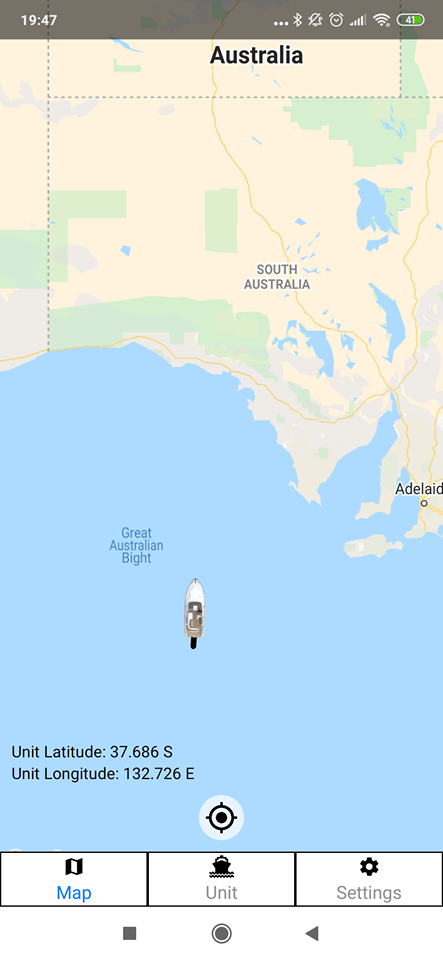
\includegraphics[scale=0.2]{graphic/MapView}
    \caption{MapView}
    \source{Opracowanie własne}
    \label{fig:MapView}
\end{figure}

\begin{figure}[H]
  \centering
    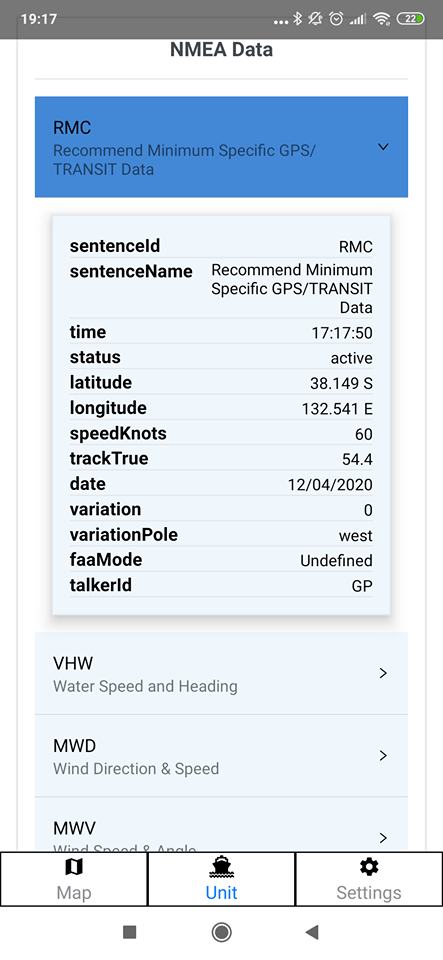
\includegraphics[scale=0.2]{graphic/UnitView}
    \caption{UnitView}
    \source{Opracowanie własne}
    \label{fig:UnitView}
\end{figure}

\begin{figure}[H]
  \centering
    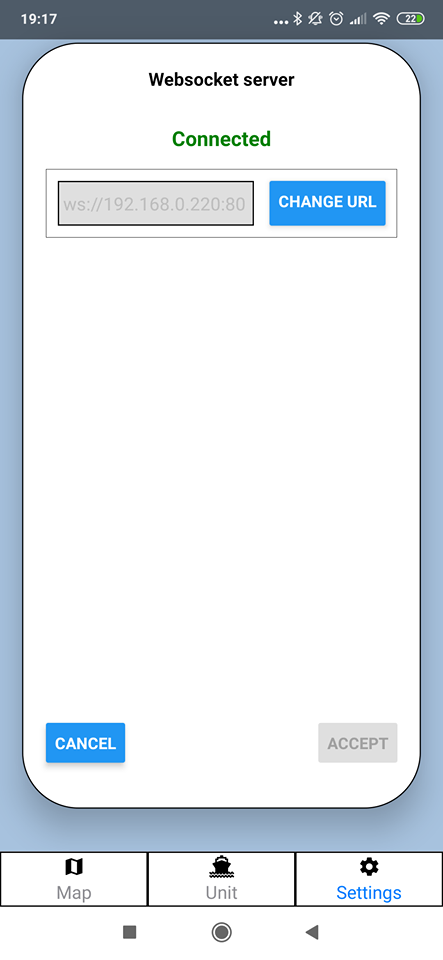
\includegraphics[scale=0.2]{graphic/Settings}
    \caption{SettingsView}
    \source{Opracowanie własne}
    \label{fig:SettingsView}
\end{figure}

%\rysunek{MapView}
%{MapView \label{fig:MapView}}
%{Opracowanie własne}
%
%\rysunek{UnitView}
%{UnitView \label{fig:UnitView}}
%{Opracowanie własne}
%
%\rysunek{Settings}
%{Settings \label{fig:SettingsView}}
%{Opracowanie własne}

	Taki podział komponentów pozwala na intuicyjne odczytywanie danych dotyczących położenia, dzięki wykorzystaniu map Google, oraz dokładnych odczytów poszczególnych składowych komend \textit{NMEA}. Każdy nowy format dodany do aplikacji poprzez stworzenie odpowiedniego pliku kodeka automatycznie zostanie odzwierciedlony w UnitView o ile dane otrzymywane przez aplikację taką komendę zawierają. Dzięki temu interfejs użytkownika jest łatwo rozwijalny.

% reconsilation, virtual DOM. React Native korzysta z Virtual DOMu na tej samej zasadzie co React, tylko po procesie rekonsilacji wywoływane są ponownie natywne elementy danej platformy zależnie od renderera (iOS/Android) a nie webowe. React Native używa Fiber tak samo jak ReactJS.

%\subsection{Bibliografia}
%
%Wszystkie pozycje bibliograficzne powinny być zacytowane w~treści pracy.
%
%Opisy bibliograficzne wynikają ze zwyczajów stosowanych w~różnych dziedzinach nauki lub wytycznych różnych wydawnictw. Przygotowując bibliografię powinno się więc \textbf{konsekwentnie przestrzegać} kolejności elementów opisu, jak i~sposobu ich zredagowania. Opis bibliograficzny powinien być przygotowany tak, aby możliwe było jednoznaczne określenie źródła bibliograficznego. Przy sporządzaniu bibliografii zaleca się \textbf{przyjąć kolejność alfabetyczną} względem nazwiska pierwszego autora, natomiast przy kilku pracach tego samego pierwszego autora przyjąć należy ich kolejność według daty publikacji (rosnąco). W~wypadku wykorzystania w~pracy źródeł drukowanych lub internetowych nieposiadających jawnie wskazanych autorów (np. materiały firmowe, dokumentacje), można w~spisie bibliografii wydzielić taką grupę źródeł bibliograficznych.
%
%%Przykład cytowania źródła internetowego:~\cite{Chwalowski2002}, podręcznika dostępnego w~wersji elektronicznej:~\cite{Nowacki1996,Reckdahl1997}, artykułu naukowego:~\cite{Iksinski2000} i~książki:~\cite{Honczarenko2000,Opoka2001}.
%
%Wygodne narzędzie do posługiwania się wieloma pozycjami literaturowymi stanowić może menedżer bibliografii zgodny z notacją BibTeX np. darmowy JabRef. Plik przechowujący pozycje bibliograficzne zdefiniowane dla dokumentu ma nazwę \lstinline|bibliografia.bib|. Na podstawie tego pliku LaTeX generuje spis literatury (Bibliografię). Do tego celu służy pakiet \textbf{Biber}, stanowiący następcę pakietu BibTeX, zapewniający m.in. pełne wsparcie standardu Unicode. W~przypadku użycia edytora TeXstudio współpracującego ze środowiskiem MiKTeX w~systemie Windows, może być konieczna zmiana domyślnego narzędzia bibliograficznego w~konfiguracji programu (menu: opcje/konfiguruj/zbuduj/metapolecenia), a~także jego wywołanie (menu: narzędzia/bibliografia lub skrót klawiszowy F8), a~następnie ponowna kompilacja dokumentu.  


\begin{zakonczenie}\label{chap:zakonczenie}
	Udało się stworzyć aplikację mobilną zgodną z wymaganiami pracy, pod niektórymi względami przewyższającą część dostępnych na rynku rozwiązań. Struktura kodu źródłowego pozwala na oddzielenie warstwy dekodowania danych od warstwy widoku. Dzięki temu możliwym byłoby dostarczenie biblioteki zajmującej się przetwarzaniem danych NMEA, możliwej do wykorzystania przez inne aplikacje. Najtrudniejszym zagadnieniem okazało się stworzenie jak najbardziej generycznej obsługi komend. Dodatkowe problemy sprawił również utrudniony dostęp do dokumentacji, większość dostępnej wiedzy stanowią źródła w postaci stron internetowych. 
	Interfejs użytkownika można wzbogacić o wiele informacji oraz funkcjonalności, dla przykładu - dane historyczne, możliwość ustalania własnych znaczników wraz z opisami, system alarmowy. Oprócz tego warto byłoby zapewnić możliwość pracy aplikacji w trybie offline. Dla warstwy dekodującej wsparcie dla komend protokołu NMEA 2000 oraz AIS byłoby niewątpliwym atutem.
\index{transformata}
\end{zakonczenie}

% Bibliografia
\printbibliography[heading=bibintoc]

% Spis tabel (jeżeli jest potrzebny)
\listoftables

% Spis rysunków (jeżeli jest potrzebny)
\listoffigures

% Spis kodów źródłowych (jeżeli jest potrzebny)
\listoflistings

% TODO: Przenieść generowanie do pakietu glossaries i wyemilinować potrzebę manualnego wykonywania polecenia makeindex w terminalu. !! Dyskusyjne, indeksy należy definiować w preambule lub w osobnym pliku (tak samo jak acronyms), ale pozwala na większą swobodę w definiowaniu wpisów i nie wymaga wywoływania makeindex !!

% Skorowidz (opcjonalnie), po skompilowaniu dokumentu należy użyć opcji Narzędzia -> Indeks,
% aby wygenerować wpisy, po czym powtórnie skompilować dokument.
\printindex

\end{document}
